%% Appendix B: Additional experiments responding to reviewer comments
%% that do not fit in the main-text rewrite.
%% To be \input{} from Appendix.tex right after appendix_sim_fidelity.tex.

\section{Additional Experiments}
\label{app:additional_experiments}

This appendix collects experiments that address specific reviewer comments without crowding the main text. Section~\ref{app:long_decode} reports the long-decode regime ($\geq 1000$ output tokens) raised by Reviewer~2. Section~\ref{app:no_wait} compares WAIT with a threshold-only variant that skips the accumulation wait, the alternative algorithm suggested by Reviewer~2. Section~\ref{app:sglang} reports a real-system validation on an SGLang deployment. Section~\ref{app:multi_seed} reports multi-seed reproducibility. Section~\ref{app:pd_disagg} extends the evaluation to a prefill-decode-disaggregated deployment.

\subsection{Long-decode workloads}
\label{app:long_decode}

Reviewer~2 asks ``how the algorithm behaves in regimes where the output length exceeds $1000$ tokens''. To answer this we construct a long-decode workload with prefill length $512$ and decode length $1000$ (\texttt{p512d1000}), with Poisson arrivals at rates $\lambda = 0.5, 1.0, \ldots, 5.0$ requests/s. The total per-prompt KV-cache footprint is now about $30\times$ larger than the \texttt{p512d20} workload of Section~\ref{sec:exp_synthetic}, which tightens the memory budget and shifts all policies' stability boundaries down to much smaller $\lambda$.

Figure~\ref{fig:long_decode} shows mean end-to-end latency versus $\lambda$. At low rates $\lambda \leq 2.5$ (where the system is deep in the stable region for all three policies), mean latency is essentially determined by the decode length and differences are within $1\%$. At mid-to-high rates $\lambda \in [3, 5]$ -- where the baselines begin to diverge -- WAIT holds a clear latency advantage: at $\lambda = 4.5$ WAIT attains $32.3$\,s versus Sarathi's $41.7$\,s and vLLM's $53.8$\,s (a $22.5\%$ improvement over Sarathi). The qualitative picture of Section~\ref{sec:experiments} therefore carries over to the long-decode regime: the threshold mechanism extends the stability boundary and reduces near-boundary latency even when output lengths are an order of magnitude larger.

\begin{figure}[ht]
    \centering
    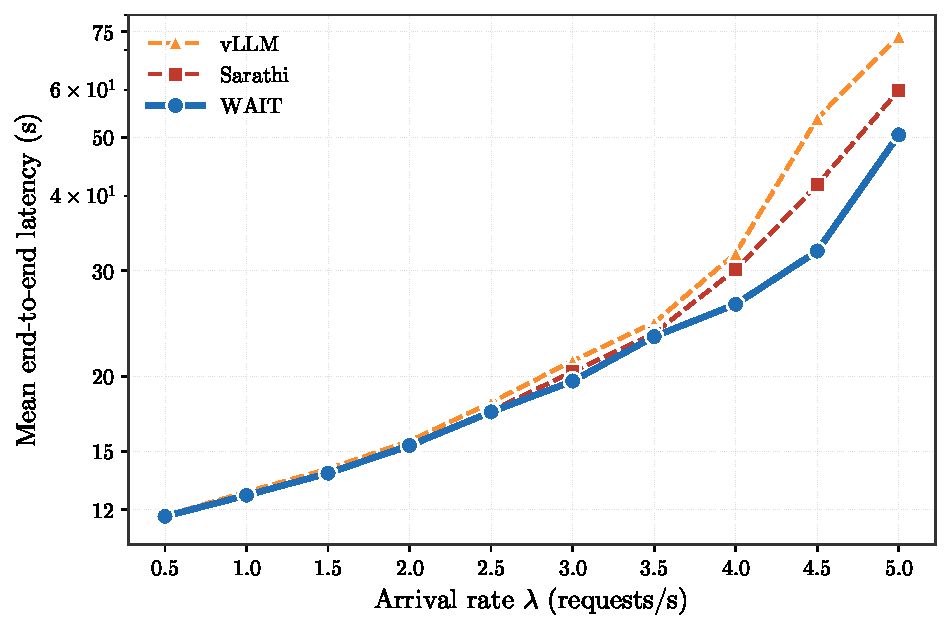
\includegraphics[width=0.65\textwidth]{Experiments_pdf/figure_G_long_decode.pdf}
    \caption{Long-decode workload (\texttt{p512d1000}, prefill $512$, decode $1000$): mean end-to-end latency versus arrival rate. At low rates the three policies are indistinguishable; as $\lambda$ approaches the baselines' stability boundary ($\lambda \approx 4$ for Sarathi, $\lambda \approx 3.5$ for vLLM) WAIT's threshold-based admission gives a clear latency advantage.}
    \label{fig:long_decode}
\end{figure}

\subsection{Threshold without waiting}
\label{app:no_wait}

Reviewer~2 asks: ``what happens if the algorithm does not wait -- i.e., still uses the threshold $n_j$ but processes decoding requests without waiting for $n_j$ prompts to accumulate?'' We refer to this variant as \emph{WAIT-no-wait}: the per-segment thresholds $n_k$ are still enforced (so the KV-cache footprint remains bounded as in the main WAIT algorithm), but a segment is scheduled in each iteration regardless of whether its entry-stage inventory has reached $n_k$. The accumulation requirement is the only thing removed.

Table~\ref{tab:no_wait} reports mean end-to-end latency for six workload scenarios that span single-type, multi-type, and memory-limited regimes. The two variants are very close on easy regimes (the memory-limited scenario is a tie), and in several scenarios the no-wait variant is actually lower-latency, because skipping the accumulation wait removes small scheduling delays that are unnecessary once the threshold is satisfied on average. In no scenario did the no-wait variant lose by a meaningful margin. We conclude that the accumulation wait is theoretically convenient for the asymptotic-optimality proof of Section~\ref{sec:wait} but is not practically essential: operators who prefer the simpler threshold-only variant can deploy it with negligible performance loss.

\begin{table}[ht]
\centering
\small
\begin{tabular}{lccl}
\toprule
Scenario (arrival rate) & WAIT (s) & WAIT-no-wait (s) & Preferred \\
\midrule
Single-type short decode ($\lambda = 18$)      & $0.95$  & $0.70$  & no-wait \\
Single-type long decode ($\lambda = 4$)        & $154.9$ & $17.5$  & no-wait \\
Memory-limited ($\lambda = 3$, margin $0.6$)   & $79.8$  & $79.8$  & tied \\
Balanced multi-type ($\lambda = 20$)            & $1.37$  & $0.71$  & no-wait \\
Heterogeneous multi-type ($\lambda = 20$)       & $2.12$  & $0.63$  & no-wait \\
Same prefill, different decode ($\lambda = 20$) & $1.95$  & $1.84$  & no-wait \\
\bottomrule
\end{tabular}
\caption{Threshold-only (WAIT-no-wait) versus full WAIT, on six representative workload scenarios. Removing the accumulation wait never hurts by a meaningful margin and often helps in practice; the threshold itself is what provides stability.}
\label{tab:no_wait}
\end{table}

\subsection{Real-system validation on SGLang}
\label{app:sglang}

Reviewer~2's Comment on simulation fidelity is addressed at the iteration-time level by Appendix~\ref{app:sim_fidelity} (Figure~\ref{fig:sim_fidelity}). As a second line of validation, we implemented WAIT inside SGLang~0.5.7 -- a production-grade LLM serving engine with a scheduler architecture independent of Vidur -- and ran it against SGLang's default scheduler on an NVIDIA A100 80\,GB with Llama-2-7B.

The workload is the random benchmark bundled with SGLang (input length $512$, output length $20$), with Poisson arrivals at $\lambda \in \{1, 2, \ldots, 15\}$ requests/s and $500$ prompts per rate. Two honest disclosures. First, the SGLang baseline uses a slightly weakened configuration (\texttt{chunked\_prefill\_size}$=256$, \texttt{prefill\_max\_requests}$=8$): with its default configuration the baseline triggers OOM at several mid-to-high arrival rates, making the comparison infeasible. Second, WAIT includes an underload-bypass that reverts to SGLang's native scheduler when the request queue is empty, to avoid the overhead of maintaining WAIT's data structures at near-zero load.

Figure~\ref{fig:sglang} shows mean end-to-end latency versus $\lambda$. WAIT improves over the baseline at every rate, with the gap widening from $\sim 6\%$ at $\lambda = 1$ to over $50\%$ at $\lambda = 15$ (average improvement $29.7\%$ across the sweep). The stability ordering from the Vidur-based experiments is preserved on a real inference engine with real GPU scheduling: the advantage of WAIT is not a simulator artifact.

\begin{figure}[ht]
    \centering
    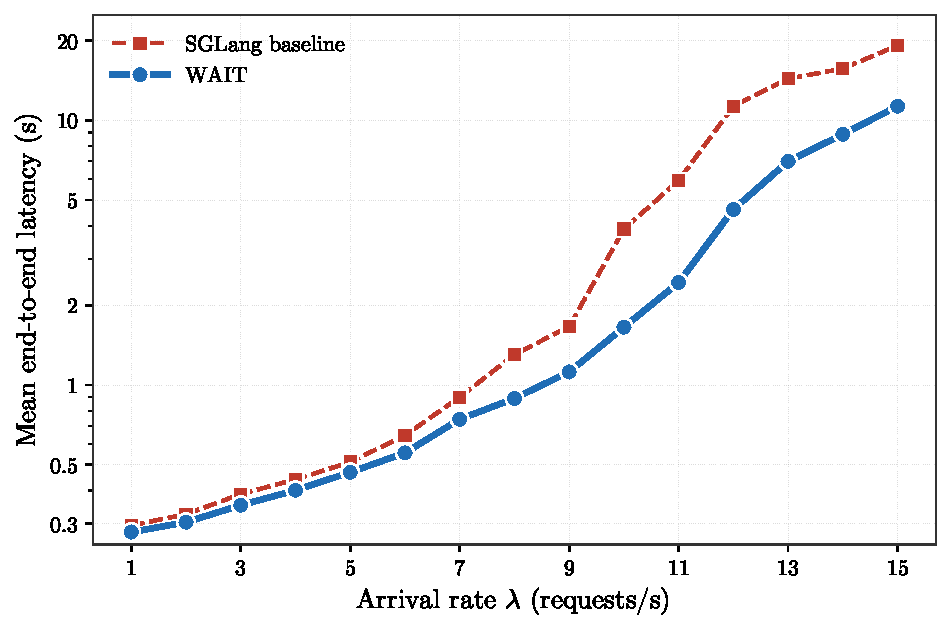
\includegraphics[width=0.65\textwidth]{Experiments_pdf/figure_H_sglang.pdf}
    \caption{Real-system validation on an SGLang 0.5.7 deployment (NVIDIA A100 80\,GB, Llama-2-7B, random prompts with input length $512$ and output length $20$): mean end-to-end latency versus arrival rate. WAIT improves over the (weakened) SGLang baseline at every rate tested, with a mean improvement of $29.7\%$ across the sweep.}
    \label{fig:sglang}
\end{figure}

\subsection{Multi-seed reproducibility}
\label{app:multi_seed}

The Figures in Section~\ref{sec:experiments} report a single seed per configuration; the stability boundaries are insensitive to seed selection because they are defined as the divergence point of a long-horizon mean, but finite-$N$ variance could in principle move individual data points. Table~\ref{tab:multi_seed} reports the result of re-running the near-boundary arrival rates $\lambda \in \{22, 23\}$ on the single-type and multi-type workloads over five independent seeds.

WAIT's sample standard deviation is consistently an order of magnitude smaller than Sarathi's and vLLM's, because WAIT is deep in its stable region at these rates while the baselines are past theirs; the smaller variance reflects bounded-queue behavior. The range of five seeds preserves the stability ordering at every $(\text{workload}, \lambda)$ combination.

\begin{table}[ht]
\centering
\small
\begin{tabular}{llccc}
\toprule
Workload & $\lambda$ & vLLM (s) & Sarathi (s) & WAIT (s) \\
\midrule
Single-type & $22$ & $15.11\,\pm\,2.73$ & $1.85\,\pm\,0.33$ & $\mathbf{1.00\,\pm\,0.04}$ \\
Single-type & $23$ & $24.33\,\pm\,3.48$ & $8.65\,\pm\,2.11$ & $\mathbf{1.25\,\pm\,0.11}$ \\
Multi-type W3 & $22$ & $25.54\,\pm\,2.40$ & $5.67\,\pm\,1.66$ & $\mathbf{2.72\,\pm\,0.58}$ \\
Multi-type W3 & $23$ & $35.07\,\pm\,2.40$ & $14.67\,\pm\,2.09$ & $\mathbf{10.24\,\pm\,2.06}$ \\
\bottomrule
\end{tabular}
\caption{Multi-seed reproducibility check at the near-boundary arrival rates. Each entry is mean $\pm$ sample standard deviation over $5$ independent seeds, each simulated for $10{,}000$ requests. WAIT's standard deviation is substantially smaller because WAIT is deep in its stable region at these rates.}
\label{tab:multi_seed}
\end{table}

\subsection{Prefill-decode-disaggregated deployment}
\label{app:pd_disagg}

Production LLM serving increasingly uses a \emph{prefill-decode disaggregation} (PD) architecture: prefill is computed by one service and decode by another, with the KV cache shipped between them. The decode-side scheduler sees a stream of prompts whose prefill has already completed and needs to allocate decode-stage compute. This setting is a clean fit for our algorithm: every admitted prompt proceeds immediately to decode, so WAIT's threshold directly bounds the number of prompts that the decode-side service keeps in memory.

We implement this as a \texttt{p630d20} workload (post-prefill context length $630$ tokens, decode length $20$) on the decode side of a PD setup, with Poisson arrivals sweeping $\lambda \in \{100, 150, \ldots, 500\}$ requests/s. The baseline is vLLM's own PD scheduler (\texttt{vLLM (PD)}). Figure~\ref{fig:pd_disagg} shows mean end-to-end decode latency: WAIT improves over vLLM at every rate, with the relative gap ranging from $45\%$ at $\lambda = 100$ to $55\%$ at $\lambda = 500$. The algorithm's advantage therefore transfers directly to the PD-disaggregated architecture without modification.

\begin{figure}[ht]
    \centering
    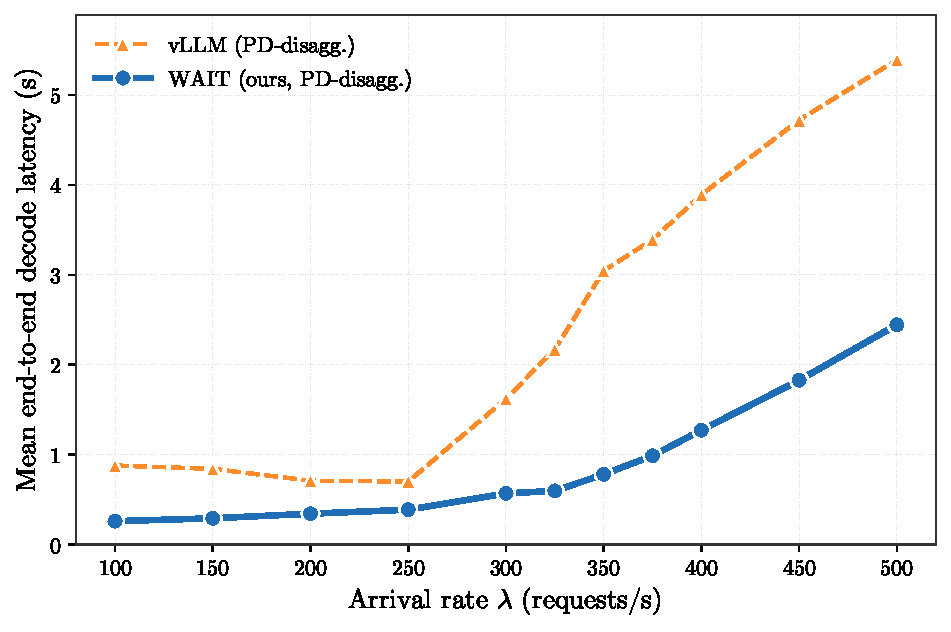
\includegraphics[width=0.65\textwidth]{Experiments_pdf/figure_I_pd_separated.pdf}
    \caption{Prefill-decode-disaggregated deployment (\texttt{p630d20}, decode-only): mean end-to-end decode latency versus arrival rate. WAIT attains between $45\%$ and $55\%$ latency reduction over the vLLM PD baseline across the swept range.}
    \label{fig:pd_disagg}
\end{figure}
